\chapter{Results, Validation, and Discussion}
\label{chap:results_validation}

\section{Introduction}

Validation in this thesis focuses on the technical correctness of the implemented prototype workflow. The objective is to verify that information can move from MQTT-originated measurements to PostgreSQL persistence, Digital Twin synchronization, machine-learning prediction, MAS decision support, dashboard display, simulation, recommendation, and supervised actuator control.

The validation is not presented as an agronomic field trial. The prototype was tested in a controlled experimental context, so the results demonstrate engineering feasibility and end-to-end integration. Claims about seasonal water savings, crop yield, or long-term irrigation performance require future field experiments.

\section{Validation protocol}

The validation protocol follows scenario-based testing. Each scenario checks one part of the Digital Twin loop: sensor acquisition, database persistence, dashboard synchronization, ML inference, simulation, recommendation, MAS explainable decision support, scheduling, and actuator feedback. A scenario is considered captured when a screenshot or inserted figure is available in this chapter. Other scenarios are documented through implementation evidence in the backend, Digital Twin, interface, MAS test suite, and deployment chapters.

\section{Test environment}

The prototype environment includes the Libelium sensing setup, XBee/Raspberry Pi gateway flow, MQTT communication, FastAPI backend, PostgreSQL database, separated Random Forest ML service, MAS service, Next.js dashboard, Flutter mobile access, WeMos actuator, and controlled pump command workflow. Docker Compose is used to coordinate the documented runtime services during local deployment.

\section{Scenario 1: MQTT sensor acquisition}

The first scenario validates physical-to-digital communication. A sensor payload is published to the \texttt{sensors/data} topic and received through the MQTT broker. This verifies that measurements can enter the software platform through the same messaging channel used by the ingestion pipeline.

\begin{figure}[H]
    \centering
    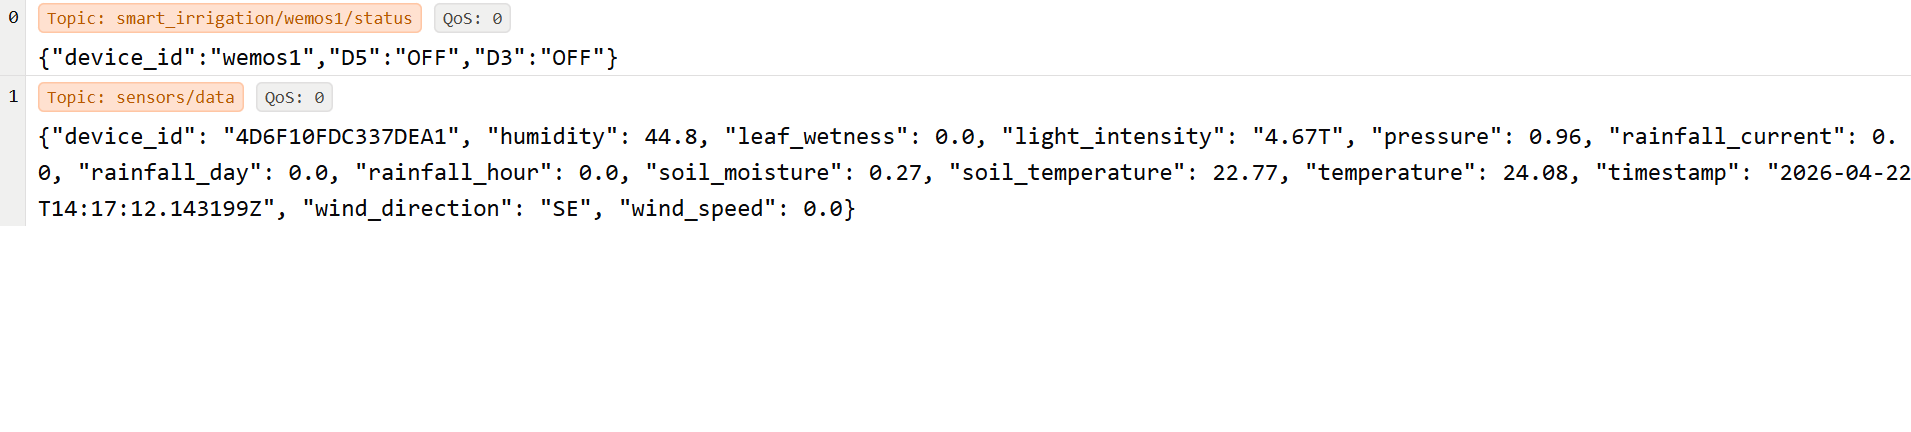
\includegraphics[width=0.9\textwidth,height=0.75\textheight,keepaspectratio]{figures/chapter_11/Figure 11.1 — Sensor MQTT message received on the sensorsdata topic.png}
    \caption{Sensor MQTT message received on the sensors/data topic.}
    \label{fig:11-1-sensor-mqtt-message-received-on-the-sensors-data-topic}
\end{figure}

Figure~\ref{fig:11-1-sensor-mqtt-message-received-on-the-sensors-data-topic} provides the captured MQTT evidence for this scenario. The result confirms that the broker receives a structured sensor message that can be consumed by the backend.

\section{Scenario 2: PostgreSQL persistence}

The second scenario validates storage of MQTT-originated measurements. After ingestion, the backend maps measurements to structured database records. The stored fields include identifiers, measurement type, value, quality information, source, and timestamp.

\begin{figure}[H]
    \centering
    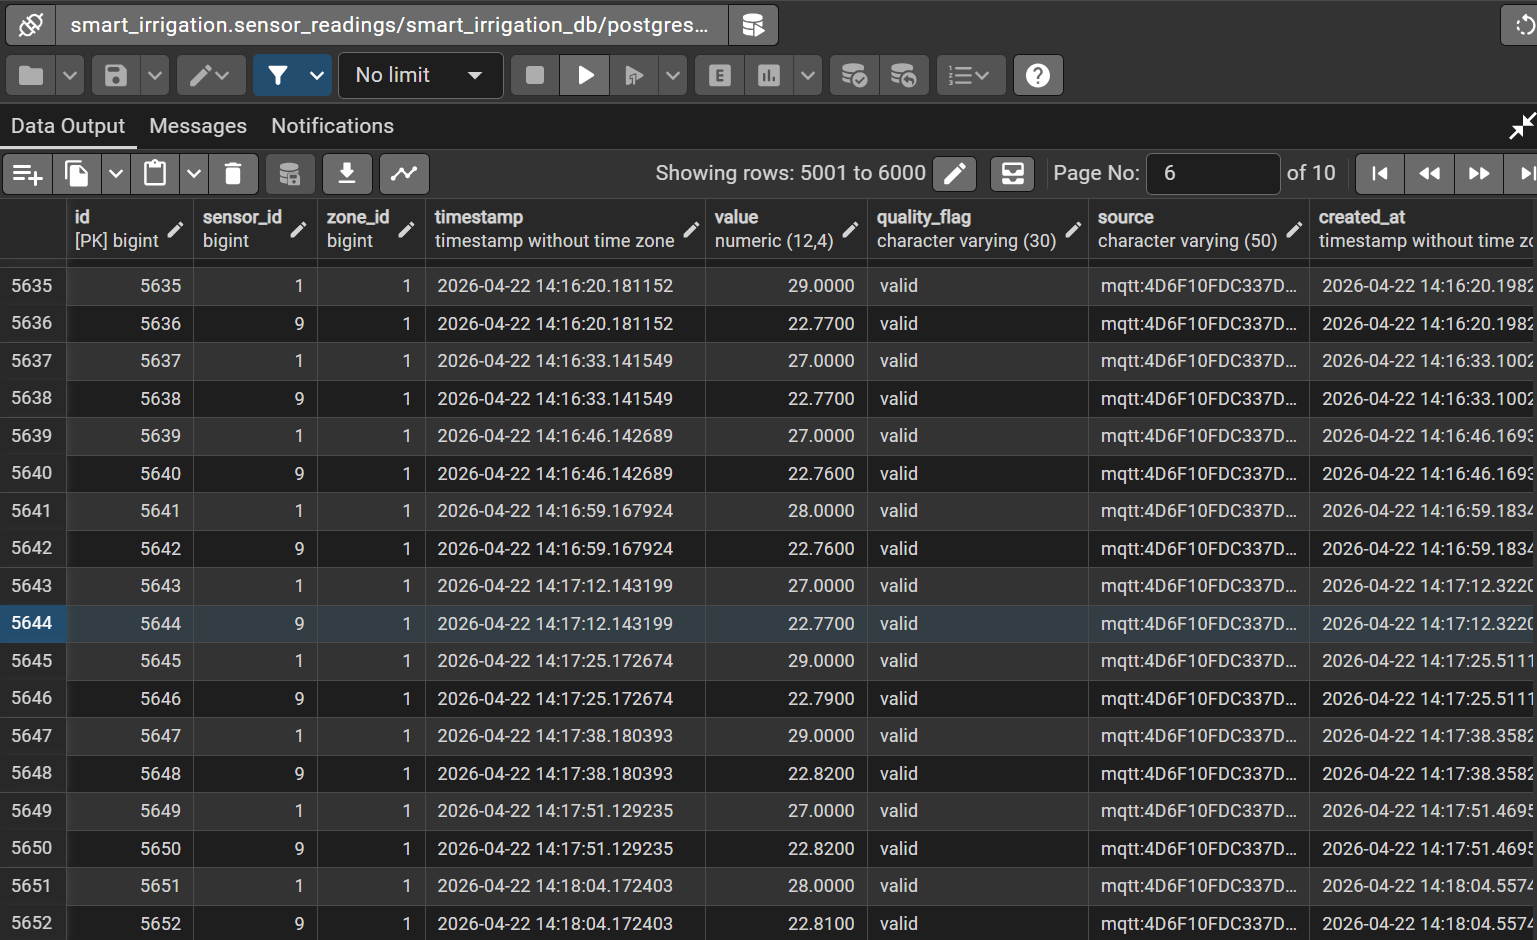
\includegraphics[width=0.9\textwidth,height=0.75\textheight,keepaspectratio]{figures/chapter_11/Figure 11.2 — Database persistence proof showing stored sensor readings from MQTT-originated data.png}
    \caption{Database persistence proof showing stored sensor readings from MQTT-originated data.}
    \label{fig:11-2-database-persistence-proof-showing-stored-sensor-readings-from-mq}
\end{figure}

Figure~\ref{fig:11-2-database-persistence-proof-showing-stored-sensor-readings-from-mq} confirms that incoming measurements are persisted in PostgreSQL. This is necessary for traceability because later Digital Twin state updates, predictions, and dashboard views depend on stored records rather than temporary MQTT messages only.

\section{Scenario 3: Dashboard synchronization}

The third scenario validates that backend state is visible to the user interface. The dashboard displays live operational data, including moisture state, zone information, sensor health, twin status, environmental values, and current recommendations.

\begin{figure}[H]
    \centering
    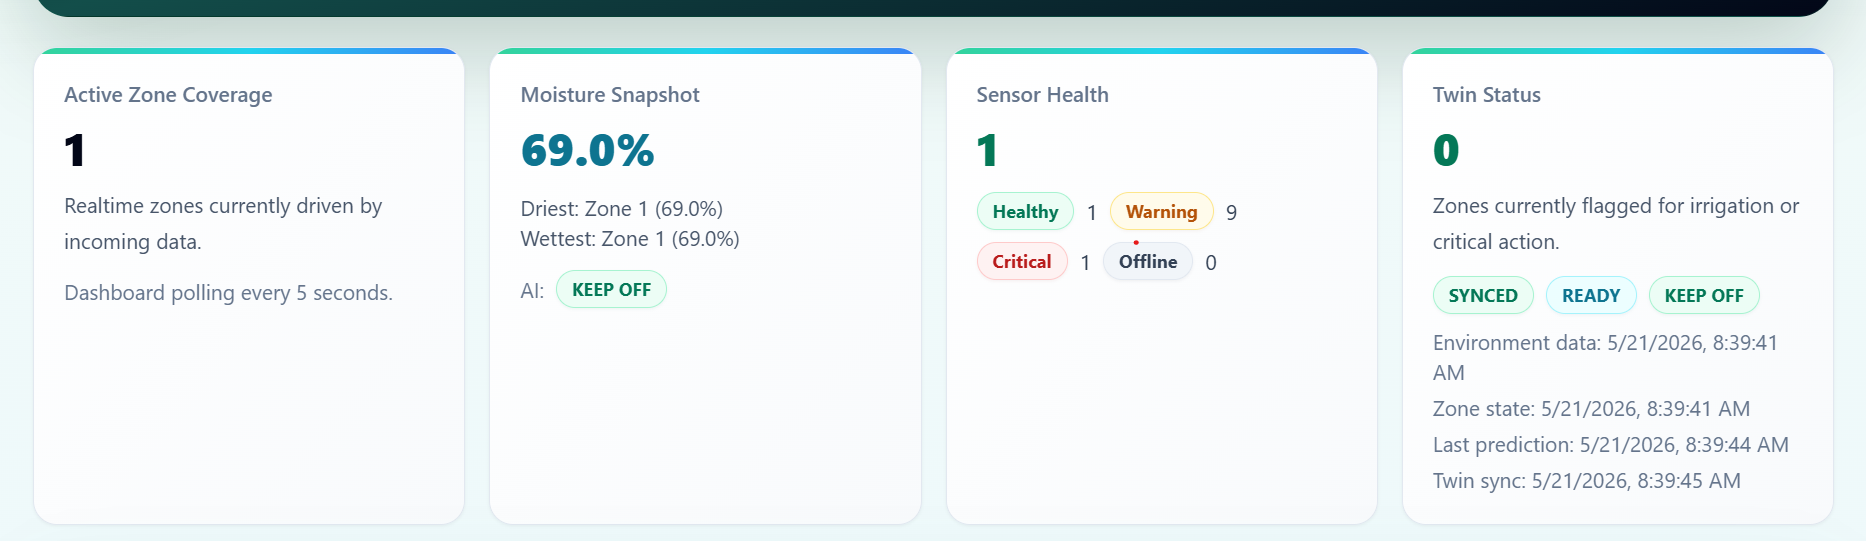
\includegraphics[width=0.9\textwidth,height=0.75\textheight,keepaspectratio]{figures/chapter_11/Figure 11.3 — Dashboard update reflecting the latest stored sensor and Digital Twin data.png}
    \caption{Dashboard update reflecting the latest stored sensor and Digital Twin data.}
    \label{fig:11-3-dashboard-update-reflecting-the-latest-stored-sensor-and-digital-}
\end{figure}

Figure~\ref{fig:11-3-dashboard-update-reflecting-the-latest-stored-sensor-and-digital-} shows that the user interface reflects stored sensor and Digital Twin data. This verifies the path from ingestion and persistence to frontend visualization.

\section{Scenario 4: Machine-learning prediction}

The ML prediction scenario validates the intelligent layer. The ML service loads Random Forest models and returns irrigation need, suggested irrigation hour, confidence values, and recommended action. The inserted evidence for this workflow is presented in the Digital Twin and machine-learning chapter through the ML health and prediction response figures, especially Figure~\ref{fig:8-4-ml-prediction-response-for-irrigation-need-and-suggested-irrigatio}.

This scenario confirms software integration between the backend and the ML service. It does not prove agronomic optimality; it proves that the trained artifacts can be loaded and used to produce runtime prediction outputs.

\section{Scenario 5: Digital Twin simulation}

The simulation scenario validates the what-if decision-support layer. The Digital Twin compares projected moisture behavior under alternative scenarios such as no irrigation, a selected irrigation duration, and an ML-selected path. The implemented simulation logic is documented in Figure~\ref{fig:8-6-what-if-simulation-logic-comparing-no-irrigation-with-irrigation-a}, while the user-facing simulation workspace and projection chart are shown in Figures~\ref{fig:9-6-digital-twin-simulation-workspace-for-running-what-if-irrigation-s} and~\ref{fig:9-7-moisture-projection-chart-comparing-no-irrigation-with-irrigation-}.

This scenario demonstrates that the platform goes beyond static monitoring. It can compare possible consequences before the user validates an irrigation action.

\section{Scenario 6: Recommendation and human validation}

The recommendation scenario validates the decision-support workflow. Recommendations are generated from Digital Twin state, prediction outputs, simulation results, forecast context, and rule-based constraints. They remain supervised: the user can inspect the recommendation, validate it, schedule it, or manually override it.

The relevant interface evidence is documented in the recommendation preview and validated-decisions figures in Chapter~\ref{chap:interfaces_control}. This confirms that the prototype exposes the decision state to the user rather than hiding the decision inside a black-box service.

\section{Scenario 7: Pump command and actuator feedback}

The actuator scenario validates the digital-to-physical part of the loop. Commands such as \texttt{ON\_D5} and \texttt{OFF\_D5} are published to the actuator command topic, while the WeMos returns status feedback on \texttt{smart\_irrigation/wemos1/status}. The payload structures for this workflow are documented in Chapter~\ref{chap:backend_database_iot} through the actuator command and WeMos status payload figures.

The current thesis evidence supports the command and feedback design through payload, backend, and interface documentation. A longer physical-actuator campaign with repeated ON/OFF cycles, timing measurements, and dedicated status screenshots remains future validation work.

\section{Scenario 8: MAS explainable irrigation decision}

The MAS scenario validates the explainable decision-support service at service level. The endpoint \texttt{/mas/decision} receives a field context and returns a structured response containing decision, explanation, confidence, risk level, suggested hour, recommended duration, evidence, and warnings. This scenario is documented through implementation and automated tests rather than a final frontend screenshot.

The MAS tests verify three representative decision cases. In the first case, dry soil with no expected rain returns \texttt{START\_IRRIGATION} and a positive recommended duration. In the second case, dry soil with high rain probability and rainfall returns \texttt{KEEP\_OFF}, with warnings explaining that rain blocks direct irrigation. In the third case, dry soil with high wind returns \texttt{SCHEDULE\_IRRIGATION}; the safety evidence blocks \texttt{START\_IRRIGATION} while preserving the suggested hour from the ML prediction. These tests confirm that the MAS combines Digital Twin state, ML prediction, weather, water balance, agronomic note, and deterministic safety rules into a safe service-level decision.

This validation does not claim full agronomic field validation. It shows that the MAS service can execute the intended engineering behavior and produce inspectable evidence under controlled test conditions.

\section{End-to-end validation summary}

\begin{footnotesize}
\setlength{\tabcolsep}{2pt}
\begin{longtable}{@{}>{\raggedright\arraybackslash}p{0.10\textwidth}>{\raggedright\arraybackslash}p{0.22\textwidth}>{\raggedright\arraybackslash}p{0.24\textwidth}>{\raggedright\arraybackslash}p{0.18\textwidth}>{\raggedright\arraybackslash}p{0.16\textwidth}@{}}
\caption{Scenario-based validation summary}\\
\label{tab:scenario_validation_summary}\\
\toprule
Test ID & Scenario & Expected result & Evidence & Status \\
\midrule
\endfirsthead
\toprule
Test ID & Scenario & Expected result & Evidence & Status \\
\midrule
\endhead
T1 & MQTT sensor acquisition & Sensor message is received on \texttt{sensors/data}. & Figure~\ref{fig:11-1-sensor-mqtt-message-received-on-the-sensors-data-topic} & Captured \\
T2 & Database persistence & Sensor readings are stored in PostgreSQL. & Figure~\ref{fig:11-2-database-persistence-proof-showing-stored-sensor-readings-from-mq} & Captured \\
T3 & Dashboard synchronization & Dashboard reflects stored sensor and Digital Twin data. & Figure~\ref{fig:11-3-dashboard-update-reflecting-the-latest-stored-sensor-and-digital-} & Captured \\
T4 & ML prediction & Runtime response contains irrigation need, suggested hour, confidence, and action. & Figure~\ref{fig:8-4-ml-prediction-response-for-irrigation-need-and-suggested-irrigatio} & Documented in Chapter 7 \\
T5 & Digital Twin simulation & Scenario output and moisture projection are generated. & Figures~\ref{fig:8-6-what-if-simulation-logic-comparing-no-irrigation-with-irrigation-a}, \ref{fig:9-6-digital-twin-simulation-workspace-for-running-what-if-irrigation-s}, and \ref{fig:9-7-moisture-projection-chart-comparing-no-irrigation-with-irrigation-} & Documented in Chapters 7 and 8 \\
T6 & Recommendation workflow & Recommendation can be inspected and validated by the user. & Figures~\ref{fig:9-3-current-field-status-and-ai-recommendation-preview-for-the-monitor} and \ref{fig:9-9-validated-decisions-interface-for-tracking-approved-irrigation-rec} & Demonstrated through interface evidence \\
T7 & Pump command and feedback & Command is sent to the actuator topic and status feedback is received. & Figures~\ref{fig:mqtt_payload_actuator_command} and \ref{fig:mqtt_payload_wemos_status} & Documented through Chapter~\ref{chap:backend_database_iot} payload and control workflow \\
T8 & MAS explainable decision & Service returns safe decision, explanation, evidence, risk, confidence, and warnings. & \texttt{test\_mas.py} service-level tests and Chapter~7 MAS section & Implemented and tested at service level \\
T9 & Scheduled irrigation & Scheduled event can be represented and executed through the scheduler workflow. & Figure~\ref{fig:9-8-irrigation-schedules-page-for-planning-and-managing-pump-execution} & Demonstrated through schedule interface and backend workflow \\
T10 & Forecast support & Forecast workspace generates weather-aware planning information. & Figure~\ref{fig:9-5-forecast-workspace-used-to-generate-weather-aware-irrigation-plann} & Demonstrated through forecast workspace \\
\bottomrule
\end{longtable}
\end{footnotesize}

\section{Discussion of results}

The results demonstrate that the prototype implements the main technical loop required by a Digital Twin-based smart irrigation platform. Measurements can be acquired through MQTT, persisted in PostgreSQL, reflected in dashboard views, processed by the intelligent layer, evaluated through MAS decision support, and connected to decision and control workflows.

The strongest captured evidence is the path from MQTT to database and dashboard. The ML, MAS, simulation, recommendation, scheduling, and actuator-control workflows are implemented and documented through the backend, Digital Twin, interface, deployment, and service-level test evidence. Future validation should extend the physical-actuator evidence with repeated ON/OFF cycles, timing measurements, farmer interaction with MAS explanations, and longer controlled-environment runs.

\section{Comparison with literature}

Compared with low-cost MQTT irrigation prototypes, Agrio adds structured persistence, Digital Twin state, ML inference, MAS explainable evidence fusion, simulation, and user validation. Compared with ML-only irrigation systems, Agrio connects prediction outputs to dashboard workflows, recommendations, scheduling, and actuator commands. Compared with field-validated Digital Twin irrigation studies, Agrio remains less mature agronomically because it has not yet been validated across seasons, plots, or crop cycles.

\section{Limitations}

The main limitations are the controlled prototype scale, limited long-term data, absence of seasonal field validation, dataset adaptation constraints, need for sensor calibration, and limited production hardening. The MAS improves explainability and safety-aware service behavior, but its agronomic recommendations still require validation with farmers and real field conditions. The prototype also lacks satellite or UAV data assimilation and does not yet include advanced optimization methods such as reinforcement learning.

\section{Future work}

Future work should include field deployment on multiple zones, crop-specific calibration, longer data collection, model retraining from real farm data, weather and evapotranspiration refinement, MAS interface screenshots and farmer explanation testing, satellite or UAV integration, stronger cybersecurity, emergency stop mechanisms, reinforcement learning optimization, and farmer usability studies.

\section{Conclusion}

This chapter validated the implemented prototype as an end-to-end technical proof of concept. The available evidence confirms MQTT acquisition, database persistence, and dashboard synchronization, while the implementation chapters document the connected ML, MAS, simulation, recommendation, scheduling, and actuator-control workflows. The system is therefore a functional engineering prototype for Digital Twin-based smart irrigation, but field-scale agronomic validation remains future work.
